Consider a planar surface and a set of $n$ rigid objects $ \objectset=\{ \object_1, \object_2 \cdots \object_n\}$  that can rest on the surface in stable poses $p_i \in \Pspace_i \subset SE(3)$. The arrangement space $ \Aspace = \Pspace_1 \times \Pspace_2 \ldots \times \Pspace_n $ is the Cartesian product of all $\Pspace_i$, where $ \arrangement = (\pose_1, \ldots, \pose_n) \in \Aspace $. In valid arrangements $ \Afree \subset \Aspace$, the objects are pairwise disjoint.

\begin{wrapfigure}{r}{2.4in}
    % \vspace{-.3in}
	\centering
	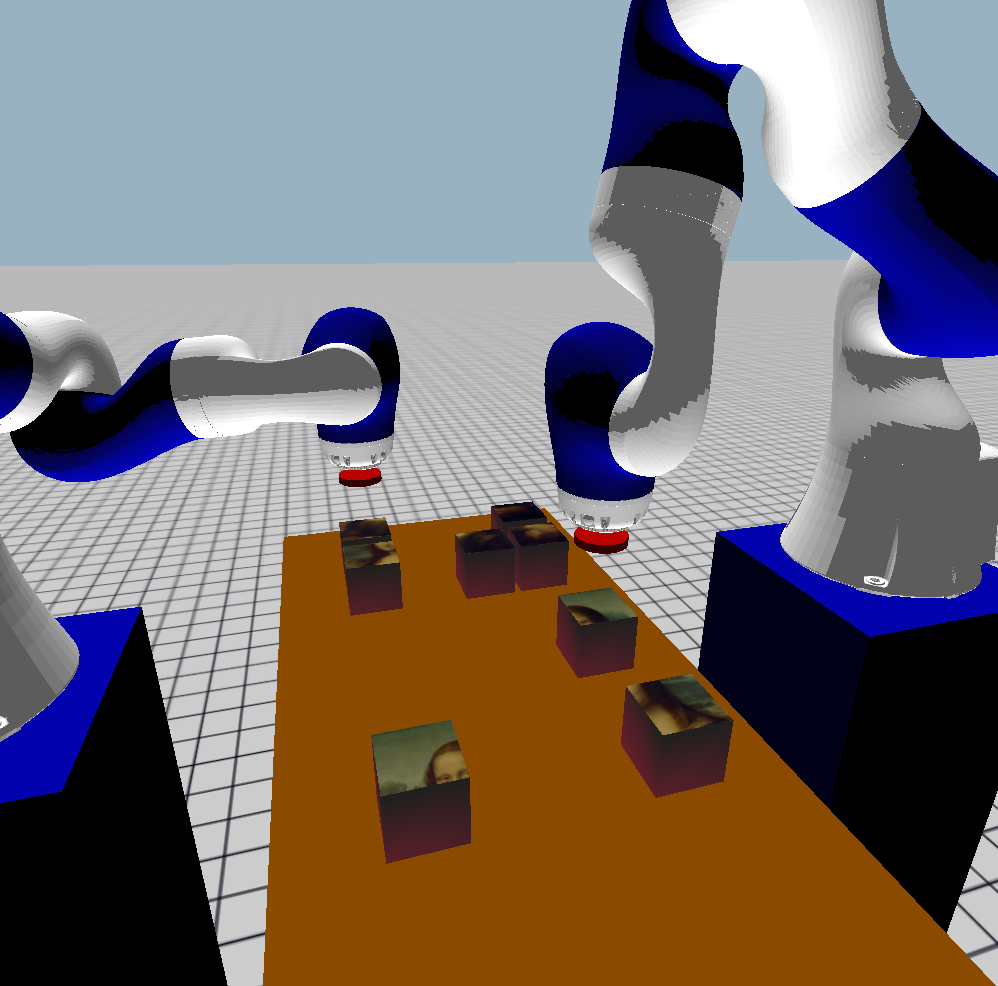
\includegraphics[width=1.115in,trim={10cm 3cm 8cm 12cm},clip]{figures/rearrangement_start}
	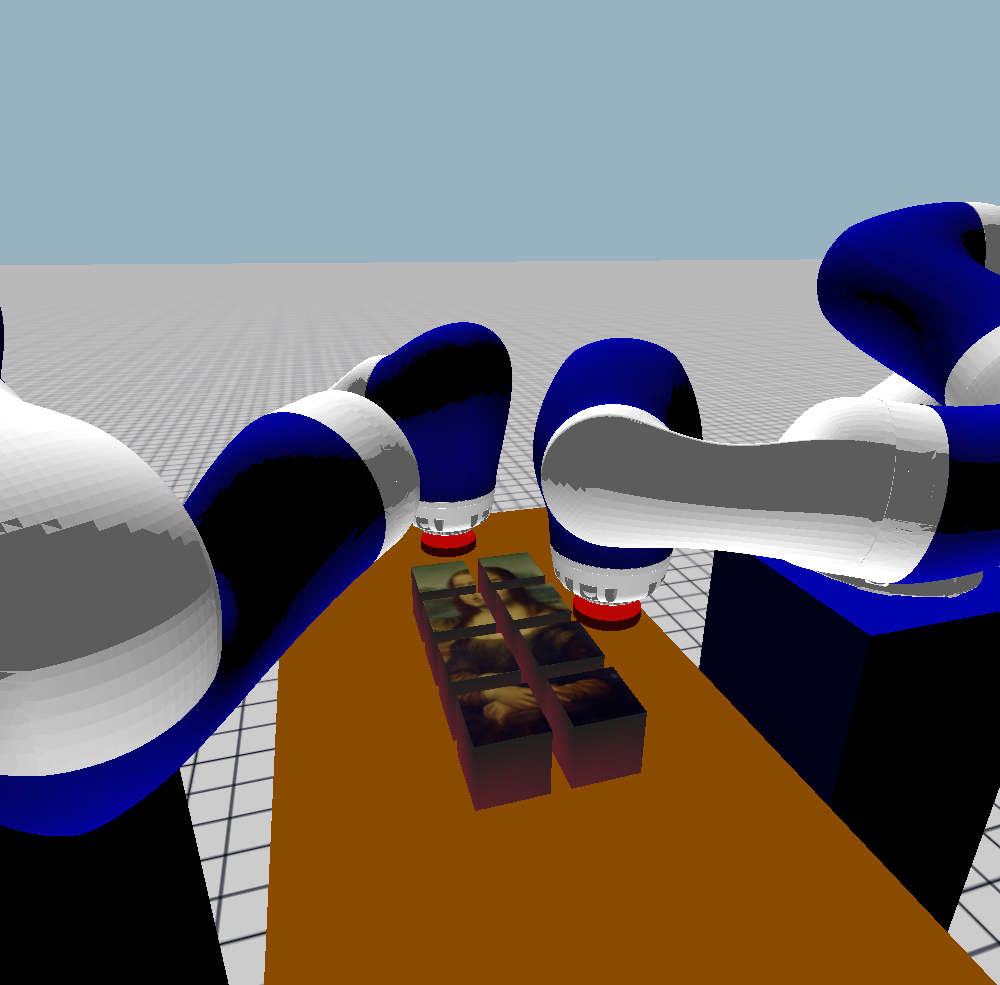
\includegraphics[width=1.115in,trim={10cm 3cm 8cm 12cm},clip]{figures/rearrangement_end}
    % \vspace{-.15in}
	\caption{An example of object rearrangement involving two robotic arms. Initial (left) and final (right) object configuration.}
	\label{fig:rearrangement}
    % \vspace{-.35in}
\end{wrapfigure}
Two robot arms $\arm^1$ and $\arm^2$ can 
% pick, raise above the surface and place the objects. 
pick and place the objects from and to the surface.
% \kiril{The last statement is unclear, particularly the purpose of the word "raise". Can it be rewritten into "...can pick and place objects from and to the surface."?}  
% THE OLD SENTENCE$\cfree^k$ is the set of collision-free configurations for arm $ \arm^k $, where $ q^k \in \cfree^k %\subset \reals^d $ (while ignoring possible collisions with  objects or the other arm).
$\cfree^k$ is the set of collision-free configurations for arm $\arm^k$ (while ignoring possible collisions with  objects or the other arm), and is assumed here to be a subset of $\reals^d $.
A path for $\arm^k$ is denoted as $ \pi^k : [0,1] \rightarrow \cfree^k$ and includes picking and placing actions.  Let $ \cfree^i(\pi^j) $ represent the collision free $\mathbb{C}$-space for $\arm^i$, given that $\arm^j$ moves along $\pi^j $. This is a function of the paths' parametrization. The space of dual-arm paths $\mathcal{D}$ denotes pairs of paths for the two arms: $D = (\pi^1,\pi^2) \in \mathcal{D}$. Then, $\arrangement(\ainit, D)$ is the resulting arrangement when the objects are at $\ainit$ and moved according to $D$.   Let $ \cost(D) : \mathcal{D} \rightarrow \reals $ be a cost function over dual-arm paths. 

% \vspace{-.1in}
{\definition [Optimal Dual-arm Rearrangement] Given arms $\arm^1$, $\arm^2$ and objects $\objectset$ to be moved from initial arrangement $ \ainit \in \Afree$ to target arrangement $ \atarget \in \Afree $, the optimal dual-arm rearrangement problem asks for a dual-arm path $D^* \in \mathcal{D}$, which satisfies the following constraint:

% \vspace{-.15in} 
\begin{equation}
% D^* =  (\pi^{*1}, \pi^{*2}) \ |\ \arrangement(\ainit, D^*) = \atarget \textrm{ and } \pi^{*i} \in \cfree^i(\pi^{*j}) \vspace{-.05in}
\label{eq:dualarm_constraint}
\end{equation}
\noindent and optimizes a cost function: $D^* = \underset{ \forall D \in \mathcal{D}}{ \mathtt{argmin} } \ \cost(D).$}

A set of assumptions are introduced to deal with the problem's combinatorics. The reachable task-space $\taskspace^k \subset SE(3)$ of arm $\arm^k$ is the set of $SE(3)$ poses that objects attached to the arm's end effector can acquire.

% \vspace{-.15in}
\commentdel{
{\textbf{Assumption} [Reachability] All objects are reachable by both arms at $\ainit$ and $\atarget$: $\forall\ \pose_i \in \ainit \textrm{ and } \forall\ \pose_j \in \atarget \textrm{ and } \forall\ k \in [1,2]: \pose_i, \pose_j \subset \taskspace^k $.}
}

Let the ordered set of objects moved during the arm path $ \pi^i $ be denoted as $ \moveset(\pi^k) $. In general, an object can appear many times in $ \moveset(\pi^k) $. The current work, however, focuses on monotone instances, where each object is moved once.

% \vspace{-.15in}
{\assumption [Monotonicity] There are dual-arm paths $D = (\pi^1,\pi^2)$ that satisfy Eq. \ref{eq:dualarm_constraint}, where each object $ \object_i \in \objectset $ appears once in $\moveset(\pi^1)$ or $ \moveset(\pi^2)$.}

\commentadd{
For the problem to be solvable, all objects are reachable by at least one arm at both $\ainit$ and $\atarget$: $\forall\ \pose_i \in \ainit \textrm{ and } \forall\ \pose_j \in \atarget \textrm{ and } \exists\ k \in [1,2]: \pose_i, \pose_j \subset \taskspace^k $.
}
The focus will be on simultaneous execution of transfer and move paths. 

\noindent\textbf{Transfers:} Dual-arm paths $T(\pi^1_i,\pi^2_i) \in \mathcal{D}$, where $ \moveset(\pi^k_i) =  \object^k_i $ and each $m^k$:
\begin{myitem}
\item[$-$]\ \ starts the path in contact with an object $\object^k_i$ at its initial pose in $\ainit$,
\item[$-$]\ \ and completes it in contact with object $ \object^k_i $ at its final pose in $\atarget$. 
\end{myitem}

\noindent\textbf{Moves or Transits:} Paths $M(\pi^1_{i\rightarrow i^{\prime}},\pi^2_{i\rightarrow i^{\prime}}) \in \mathcal{D}$, $ \moveset(\pi^1_{i\rightarrow i^{\prime}}) = \emptyset $, and each $\arm^k$:
\begin{myitem}
\item[$-$]\ \  starts in contact with object $\object^k_i$ at its final pose in $\atarget$,
\item[$-$]\ \  and completes it in contact with object $\object^k_{i^{\prime}}$ at its initial pose in $\ainit$.
\end{myitem}

% \vspace{-.1in}
{\assumption [Synchronicity] Consider dual-arm paths, which can be decomposed into a sequence of simultaneous transfers and moves for both arms:
% \vspace{-.1in}
\begin{equation}
D=\left(T(\pi^1_1,\pi^2_1),M(\pi^1_{1\rightarrow 2},\pi^2_{1\rightarrow 2}), \ldots , M(\pi^1_{\ell-1\rightarrow \ell},\pi^2_{\ell-1\rightarrow \ell}), T(\pi^1_\ell,\pi^2_\ell)\right).
% \vspace{-.05in}
\label{eq:synchronicity}
\end{equation}}
\noindent For simplicity, Eq.~\ref{eq:synchronicity} does not include an initial move from $q^k_{\rm safe} \in \cfree^k$ and a final move back to $q^k_{\rm safe}$. An odd number of objects can also be easily handled. Then, the sequence of object pairs moved during a dual-arm path as in Eq. \ref{eq:synchronicity} is: 
% \vspace{-.1in} 
% $$ \scoma(D) = \left(  \coma_i = (\object_i^1,\object_i^2) \ |\ i,j\in [1,\cdots,\ell], \bigcup_i (\object_i^1 \cup \object_i^2) = \objectset, \object_i^1 \cap \object_j^1 = \object_i^2 \cap \object_j^2 = \emptyset \right). \vspace{-.15in}$$
$$ \scoma(D) = \left(  \coma_i = (\object_i^1,\object_i^2) \ |\ i,j\in [1\cdots \ell], \bigcup_i (\object_i^1 \cup \object_i^2) = \objectset, \forall k,k'\in[1,2], \object_i^k \neq \object_j^{k'} \right). $$

\noindent Given the pairs of objects $\coma_i$, it is possible to express a transfer as $T(\coma_i)$ and a move as $M(\coma_{i\rightarrow j})$.  Then, $D(\scoma)$ is the synchronous, monotone dual-arm path due to $\scoma = (\coma_1, \ldots, \coma_{\ell})$, i.e., $D(\scoma) = (T(\coma_1),M(\coma_{1\rightarrow 2}),\ldots,M(\coma_{\ell-1\rightarrow \ell}),T(\coma_\ell)).$

% \vspace{-.1in}
{\assumption [Object Non-Interactivity] There are collision-free transfers $T(\coma_i)$ and moves $M(\coma_{i\rightarrow i^{\prime}})$ regardless of the object poses in $\ainit$ and $\atarget$.}
\commentadd{This entails that there is no interaction between the $n$ resting objects and the arms during transits. Similarly, there are no interactions between the arm-object system and the $n-2$ resting objects during the transfers. Collisions involving the arms, static obstacles and picked objects are always considered.}
\commentdel{
This assumption is valid in tabletop setups where the arms can raise the picked objects above the resting surface. 
% Furthermore, this assumption implies that transfers and moves involving object poses in $\ainit, \atarget$ are always feasible and the challenge is deciding the appropriate sequence of object-to-arm assignments.
This assumption lets the study focus on the challenge of deciding the appropriate sequence of object-to-arm assignments.
}

The metric this work focuses on relates to makespan and minimizes the sum of the longest distances traveled by the arms in each synchronized operation. Let $ \| \pi^k \| $ denote the Euclidean arc length in $\cfree^k  \subset \reals^d$ of path $ \pi^k $. Then, for transfers $\cost( T(\pi^1_i,\pi^2_i) ) = \max\{ \|\pi^1_i\|, \|\pi^2_i\| \}$. Similarly, $\cost( M(\pi^1_{i\rightarrow i^{\prime}},\pi^2_{i\rightarrow i^{\prime}}) ) = \max\{ \|\pi^1_{i\rightarrow i'}\|, \|\pi^2_{i\rightarrow i'}\| \}$. Then, over the entire dual-arm path $ \D $ define:
% \vspace{-.15in}
\begin{equation}
\cost(\D) 
% = \cost_{ T} + \cost_{ M} 
= \sum_{i=1}^{\ell}   \cost(T(\coma_i))   + \sum_{i=1}^{\ell-1}   \cost(M(\coma_{i\rightarrow i+1})). 
% \vspace{-.1in}
\label{eq:cost_function}
\end{equation}
Note that the \textit{transfer} costs do not depend on the order with which the objects are moved but only on the assignment of objects to arms. The \textit{transit} costs arise out of the specific ordering in $ \scoma(D)$. 
Then, for the setup of Definition 1 and under Assumptions 1-3, the problem is to compute the optimal sequence of object pairs $\scoma^*$ so that $D(\scoma^*)$ satisfies Eq.~\ref{eq:dualarm_constraint} and minimizes the cost of Eq.~\ref{eq:cost_function}.

\commentdel{Assumptions 2 and 3 will be partly relaxed in Section \ref{sec:integration}. Assumption 1 is also effectively relaxed to cases where at least one arm can transfer every object.}
% , given a smoothing process for achieving an asynchronous solution and a lazy motion planning process for computing transfers and moves that can be informed of object poses. 

\commentadd{
\noindent \textbf{Note on Assumptions:} This work restricts the study to a class of monotone problems that relate to a range of industrial packing and stowing applications. The monotonicity assumption is often used in manageable variants of well-studied problems~\cite{Wilson:1994fk,Halperin:2000uq}. A monotone solution also implies that every object's start and target is reachable by at least one arm. 
\cameraready{
Objects do not need to be in the commonly reachable workspace as long as the problem is monotone and solvable. Section~\ref{sec:integration} discusses a {\tt NO\_ACT} task that can deal with unbalanced object assignments between two arms. 
}

The synchronicity assumption allows to study the combinatorial challenges of the problem, which do not relate to the choice of time synchronization of different picks and placements. Section \ref{sec:integration} describes the use of $\drrtstar$\cite{Dobson:2017aa} as the underlying motion planner that can discover solutions that can synchronize arm motions for simultaneous picks, and simultaneous placements. The synchronicity assumption is relaxed through smoothing (Section \ref{sec:integration}).

The non-interactivity assumption comes up naturally in planar tabletop scenarios with top-down picks or delta robots. Such scenarios are popular in industrial settings. Once the object is raised from the resting surface, transporting it to its target does not introduce interactions with the other resting objects. This assumption is also relaxed in Section \ref{sec:integration}, with a lazy variant of the proposed method. Once a complete candidate solution is obtained, collision checking can be done with everything in the scene.

Overall, under the assumptions, the current work identifies a problem structure, which allows arguments pertaining to the search space, completeness, and optimality. Nevertheless, the smoothed, lazy variant of the proposed method will still return effective solutions in practice, even if these assumptions do not hold.

% The validation of the final candidate solution enforces that the algorithm keeps trying till a collision-free solution is found. The assumptions enable the current work to study in detail the problem, which is otherwise mostly intractable. 


}